\section{Results and Discussion}

\subsection{Diffusion}

\begin{enumerate}

    \item Data Curation and Feature Selection
    
    \begin{enumerate}

        \item Using cases which had target variables, the EnsembleModelFeatureSelector routine from MAST-ML was used to produce a learning curve from a random forest regressor. We selected 25 from 1,127 features from Figure~\ref{diffusion_learning_curve} because the mean average error (MAE) does not significantly decrease beyond 25 features.

        \begin{figure}[H]
        \centering
        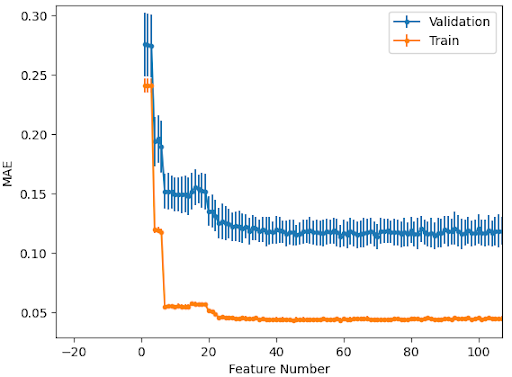
\includegraphics[width=0.95\textwidth]{figures/diffusion_learning_curve.png}
        \caption{Learning curve}
        \label{diffusion_learning_curve}
        \end{figure}
    
    \end{enumerate}
    
    \item Chemical Assessment

    \begin{enumerate}

        \item Data are aggregated and a violin plot is generated for the left out data for our $D$ score (Figure~\ref{diffusion_chemical}). We show that intuitively dissimilar materials to the Original data set, such as noble gases, are to the very right of the figure. Similar materials like transition metals are closer to the original data.

        \begin{figure}[H]
        \centering
        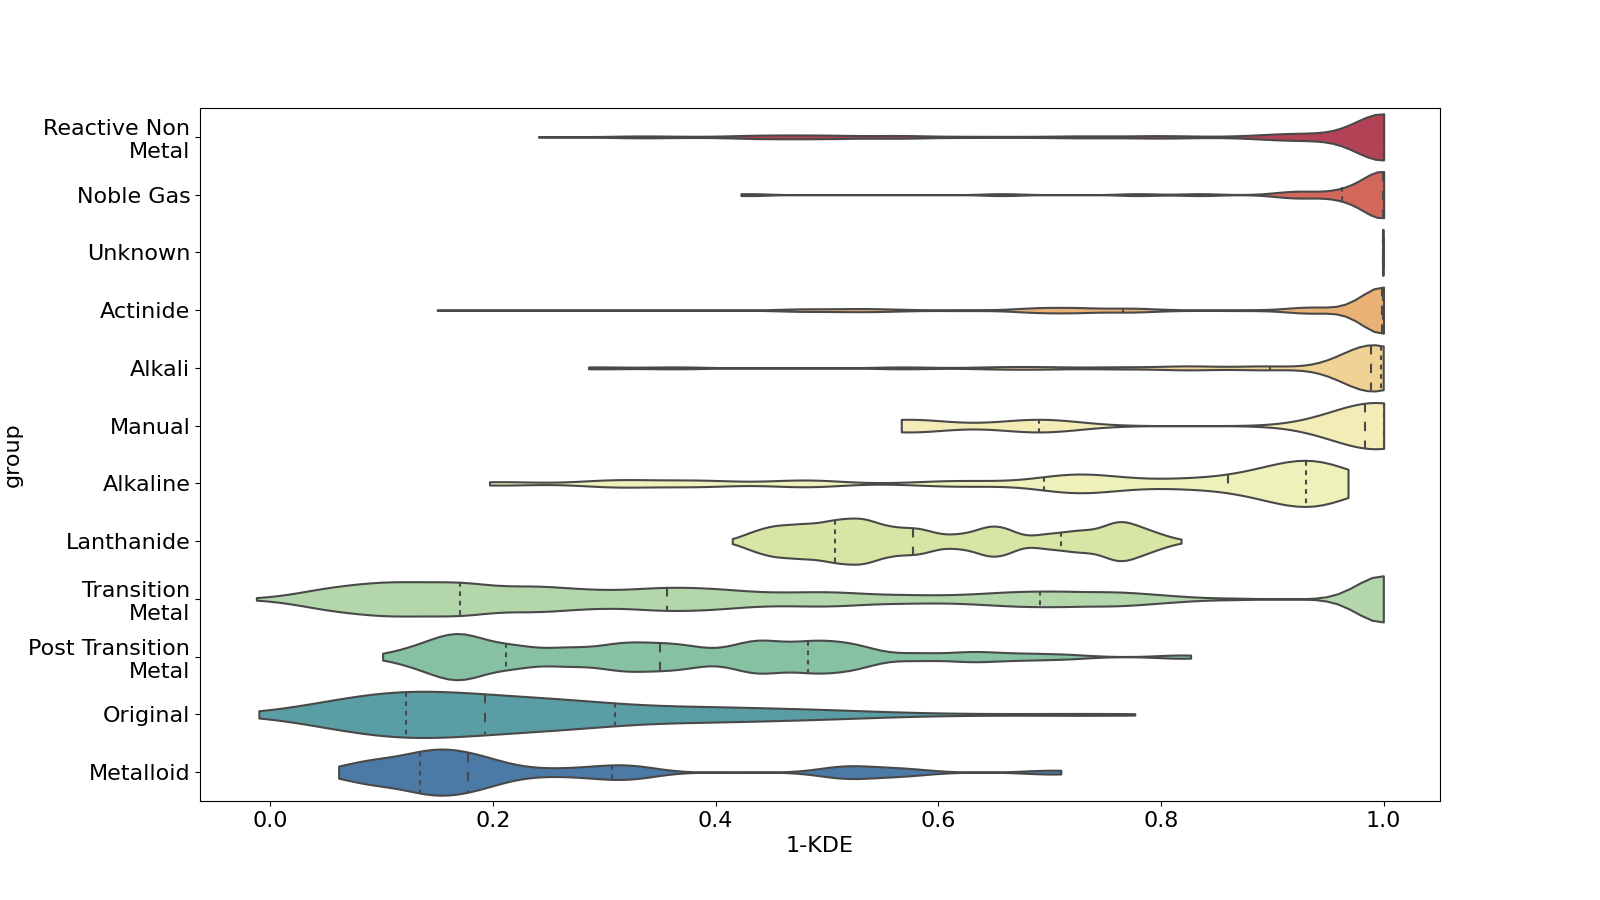
\includegraphics[width=0.95\textwidth]{figures/diffusion_chemical.png}
        \caption{Violin}
        \label{diffusion_chemical}
        \end{figure}

        \item From the domains assigned in our methods section, we acquire the PR curve shown in Figure~\ref{diffusion_chemical_pr}.

        \begin{figure}[H]
        \centering
        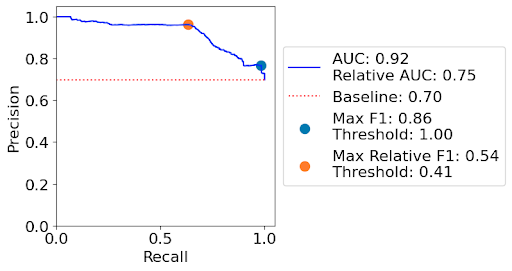
\includegraphics[width=0.95\textwidth]{figures/diffusion_chemical_pr.png}
        \caption{PR - Need to update this figure. Acts as placeholder.}
        \label{diffusion_chemical_pr}
        \end{figure}
        
    \end{enumerate}
    
    \item Numerical Single Assessment

    \begin{enumerate}

        \item Aggregated data from single numerical tests are shown in Figure~\ref{diffusion_single}. We show that our residuals grow as our $D$ score increases.

        \begin{figure}[H]
        \centering
        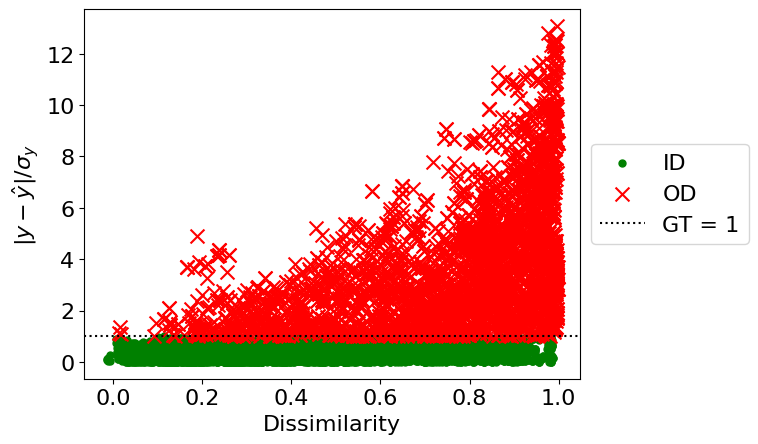
\includegraphics[width=0.95\textwidth]{figures/diffusion_single.png}
        \caption{Numerical}
        \label{diffusion_single}
        \end{figure}

        \item The associated precision recall curve is shown in Figure~\ref{diffusion_single_pr}.

        \begin{figure}[H]
        \centering
        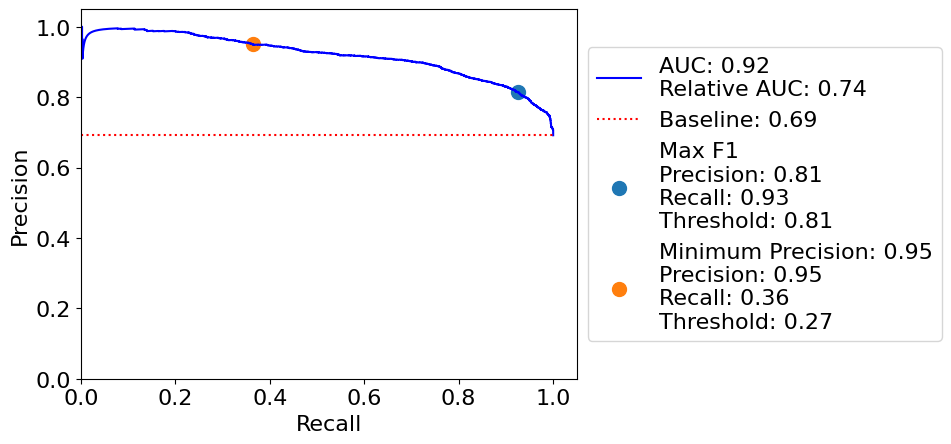
\includegraphics[width=0.95\textwidth]{figures/diffusion_single_pr.png}
        \caption{PR}
        \label{diffusion_single_pr}
        \end{figure}
    \end{enumerate}

    \item Numerical Statistical Assessment

    \begin{enumerate}
        \item We bin our data with respect to our $D$ score into 10 bins of with an equal number of points.

        \item We compare how z-score for each bin compare to a standard normal distribution (miscalibration area) and is sown in Figure~\ref{diffusion_stat}. Miscalibration area increases as data becomes increasingly dissimilar.

        \begin{figure}[H]
        \centering
        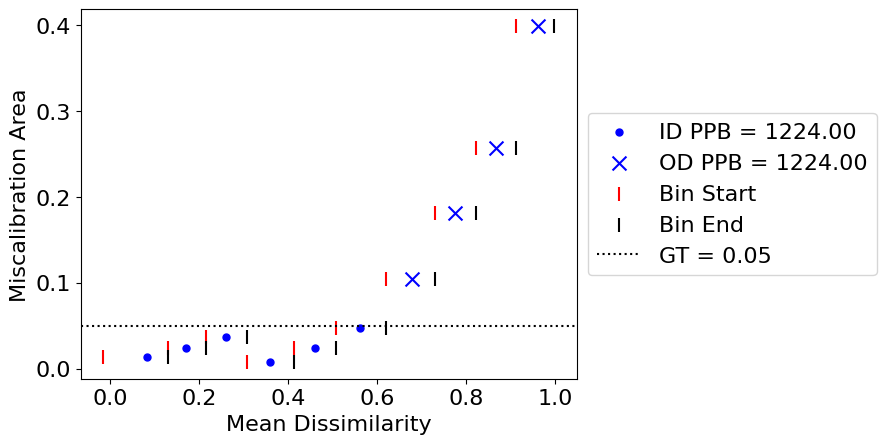
\includegraphics[width=0.95\textwidth]{figures/diffusion_stat.png}
        \caption{Numerical}
        \label{diffusion_stat}
        \end{figure}

        \item Our $D$ measure perfectly separates ID from OD data in this case in Figure~\ref{diffusion_stat_pr}.

        \begin{figure}[H]
        \centering
        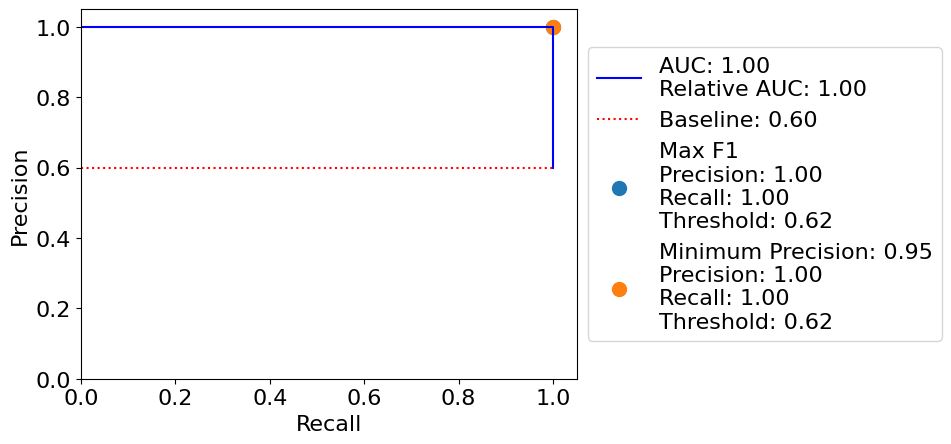
\includegraphics[width=0.95\textwidth]{figures/diffusion_stat_pr.png}
        \caption{PR}
        \label{diffusion_stat_pr}
        \end{figure}
        
    \end{enumerate}
    
\end{enumerate}

\subsection{Steel Yield Strength}

\begin{enumerate}
    \item Data Curation and Feature Selection

    \begin{enumerate}

        \item Using the original data, features were down selected from 377 to 7 features using the EnsembleModelfEatureSelector from MAST-ML. The corresponding learning curve is shown in Figure~\ref{steel_learning_curve}.


    \begin{figure}[H]
    \centering
    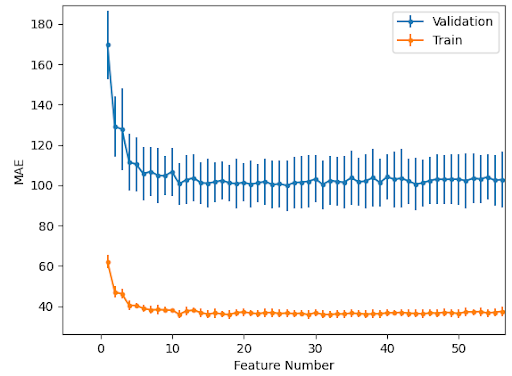
\includegraphics[width=0.95\textwidth]{figures/steel_learning_curve.png}
    \caption{Learning curve}
    \label{steel_learning_curve}
    \end{figure}
    
    \end{enumerate}
    
    \item Chemical Assessment

    \begin{enumerate}

        \item Data are aggregated and a violin plot is generated for the left out data for our $D$ score (Figure~\ref{steel_chemical}). Note that the Pertubed Original data are within the range of $D$ values and their median values align. All other data are further away from the Original data set. However, the Iron Based Far data are closer than the Copper Based and Aluminum Based sets. The observation is reasonable considering most of the Original data are iron based, but outside the range of iron weight percentages in the Original set.

        \begin{figure}[H]
        \centering
        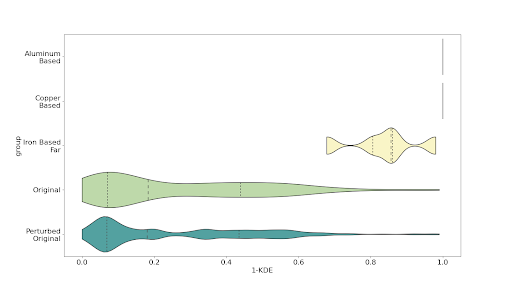
\includegraphics[width=0.95\textwidth]{figures/steel_chemical.png}
        \caption{Violin}
        \label{steel_chemical}
        \end{figure}

        \item From the domains assigned in our methods section, we acquire the PR curve shown in Figure~\ref{steel_chemical_pr}.

        \begin{figure}[H]
        \centering
        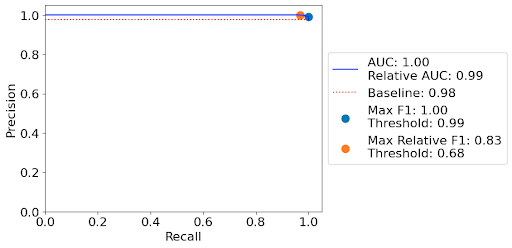
\includegraphics[width=0.95\textwidth]{figures/steel_chemical_pr.png}
        \caption{PR - Need to update this figure. Acts as placeholder.}
        \label{steel_chemical_pr}
        \end{figure}
        
    \end{enumerate}
    
    \item Numerical Single Assessment

    \begin{enumerate}

        \item Aggregated data from numerical tests are shown in Figure~\ref{steel_single}. We show that our residuals grow as our $D$ score increases.

        \begin{figure}[H]
        \centering
        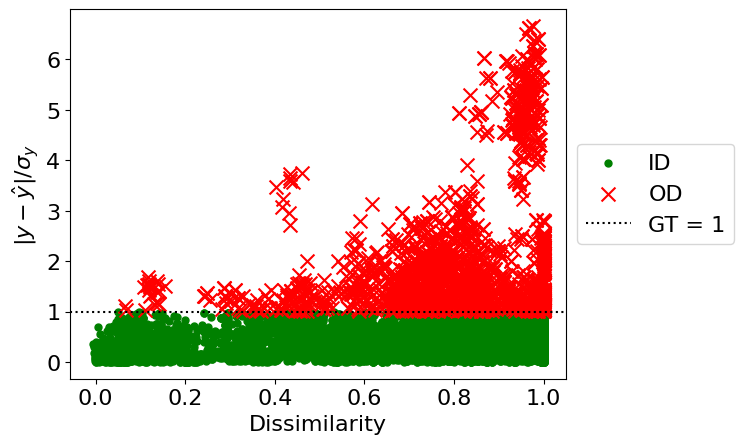
\includegraphics[width=0.95\textwidth]{figures/steel_single.png}
        \caption{Numerical}
        \label{steel_single}
        \end{figure}

        \item The associated precision recall curve is shown in Figure~\ref{steel_single_pr}.

        \begin{figure}[H]
        \centering
        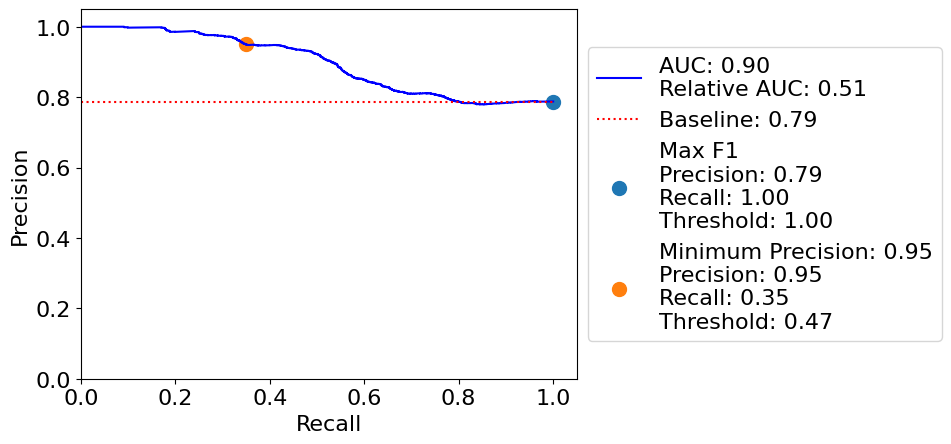
\includegraphics[width=0.95\textwidth]{figures/steel_single_pr.png}
        \caption{PR}
        \label{steel_single_pr}
        \end{figure}
    \end{enumerate}

    \item Numerical Statistical Assessment
    
    \begin{enumerate}
        \item We bin our data with respect to our $D$ score into 10 bins of with an equal number of points.

        \item We compare how z-score for each bin compare to a standard normal distribution (miscalibration area) and is sown in Figure~\ref{steel_stat}. Miscalibration area is greater to the right of around 0.5 compared to the left.

        \begin{figure}[H]
        \centering
        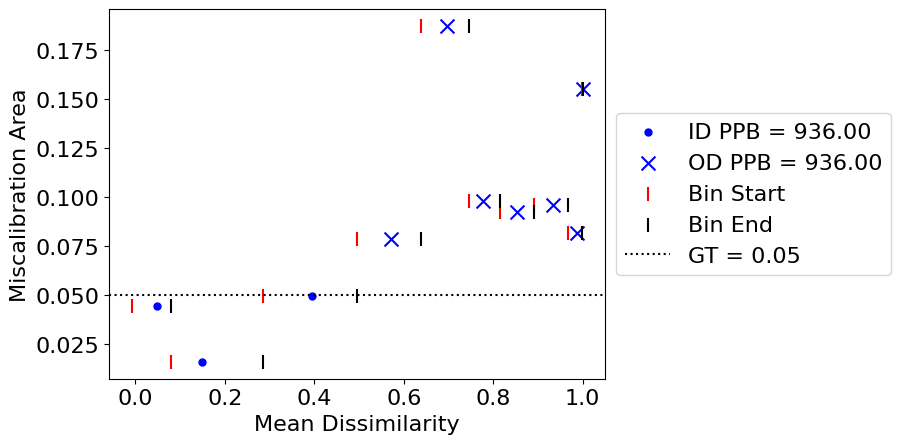
\includegraphics[width=0.95\textwidth]{figures/steel_stat.png}
        \caption{Numerical}
        \label{steel_stat}
        \end{figure}

        \item Our $D$ measure perfectly separates ID from OD data in this case in Figure~\ref{steel_stat_pr}.

        \begin{figure}[H]
        \centering
        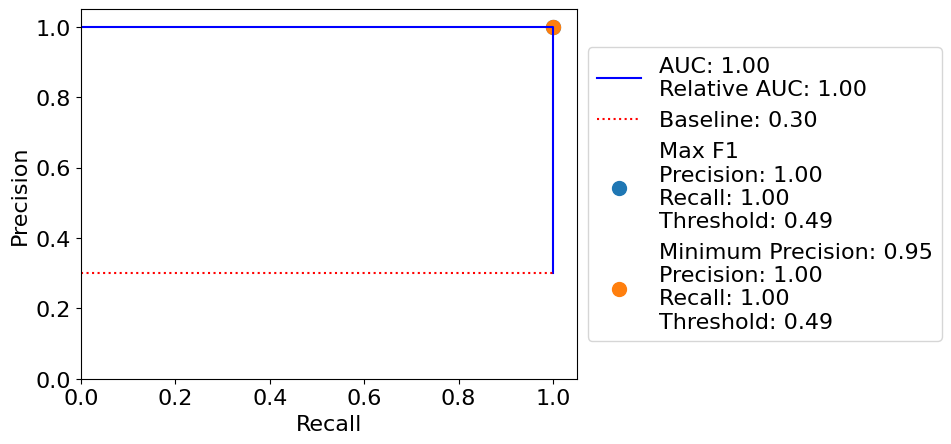
\includegraphics[width=0.95\textwidth]{figures/steel_stat_pr.png}
        \caption{PR}
        \label{steel_stat_pr}
        \end{figure}
        
    \end{enumerate}
\end{enumerate}

\subsection{Fluence}

\begin{enumerate}
    
    \item Chemical Assessment

    \begin{enumerate}

        \item Data are aggregated and a violin plot is generated for the left out data for our $D$ score (Figure~\ref{fluence_chemical}). Note that the Pertubed Original data are within the range of $D$ values and their median values align. All other data are further away from the Original data set.

        \begin{figure}[H]
        \centering
        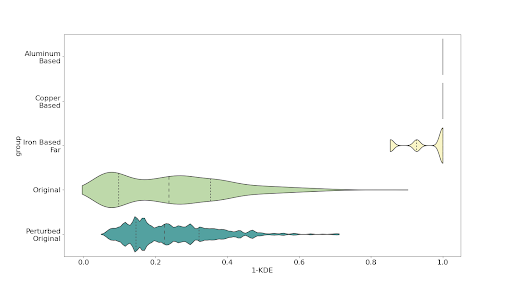
\includegraphics[width=0.95\textwidth]{figures/fluence_chemical.png}
        \caption{Violin}
        \label{fluence_chemical}
        \end{figure}

        \item From the domains assigned in our methods section, we acquire the PR curve shown in Figure~\ref{fluence_chemical_pr}.

        \begin{figure}[H]
        \centering
        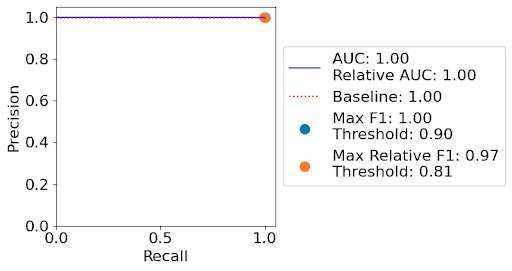
\includegraphics[width=0.95\textwidth]{figures/fluence_chemical_pr.png}
        \caption{PR - Need to update this figure. Acts as placeholder.}
        \label{fluence_chemical_pr}
        \end{figure}
        
    \end{enumerate}
    
    \item Numerical Single Assessment

    \begin{enumerate}

        \item Aggregated data from numerical tests are shown in Figure~\ref{fluence_single}. We show that our residuals grow as our $D$ score increases.

        \begin{figure}[H]
        \centering
        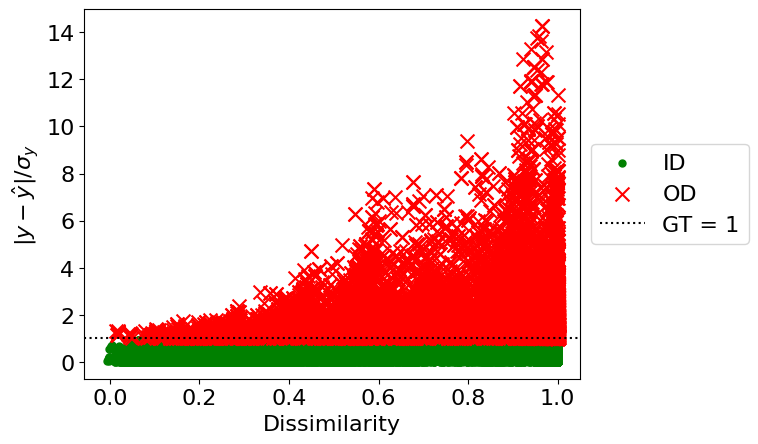
\includegraphics[width=0.95\textwidth]{figures/fluence_single.png}
        \caption{Numerical}
        \label{fluence_single}
        \end{figure}

        \item The associated precision recall curve is shown in Figure~\ref{fluence_single_pr}.

        \begin{figure}[H]
        \centering
        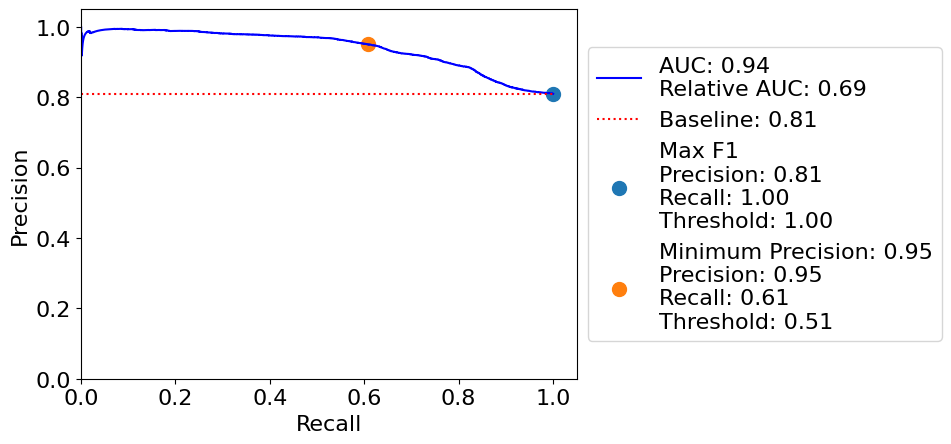
\includegraphics[width=0.95\textwidth]{figures/fluence_single_pr.png}
        \caption{PR}
        \label{fluence_single_pr}
        \end{figure}
    \end{enumerate}

    \item Numerical Statistical Assessment

    \begin{enumerate}
        \item We bin our data with respect to our $D$ score into 10 bins of with an equal number of points.

        \item We compare how z-score for each bin compare to a standard normal distribution (miscalibration area) and is sown in Figure~\ref{fluence_stat}. Miscalibration area is greater to the right of around 0.5 compared to the left.

        \begin{figure}[H]
        \centering
        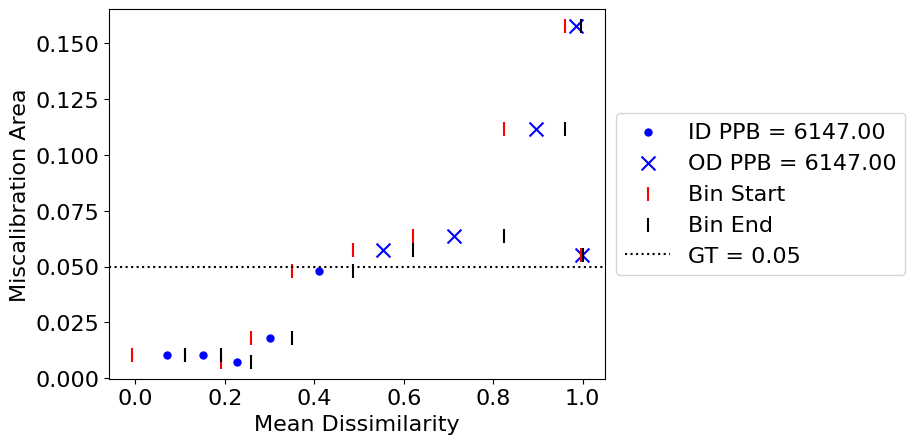
\includegraphics[width=0.95\textwidth]{figures/fluence_stat.png}
        \caption{Numerical}
        \label{fluence_stat}
        \end{figure}

        \item Our $D$ measure perfectly separates ID from OD data in this case in Figure~\ref{fluence_stat_pr}.

        \begin{figure}[H]
        \centering
        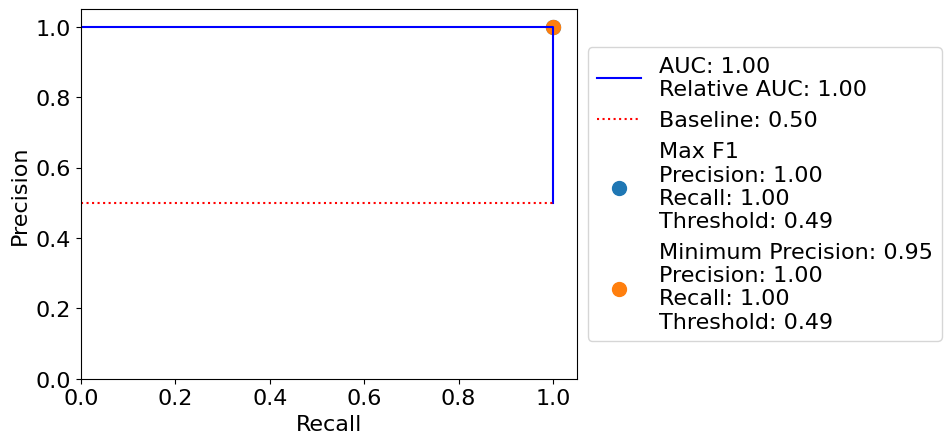
\includegraphics[width=0.95\textwidth]{figures/fluence_stat_pr.png}
        \caption{PR}
        \label{fluence_stat_pr}
        \end{figure}
        
    \end{enumerate}

\end{enumerate}

\subsection{Super Conduction}

\begin{enumerate}
    \item Chemical Assessment
    \begin{enumerate}
        \item Data are aggregated and a violin plot is generated for the left out data four our $D$ score. Figure~\ref{cond_high_chemical} has the violin plot for when we treat the majority of leave out data as $T_{low}$. As expected, our $T_{low}$ data median is near 1. 

        \begin{figure}[H]
        \centering
        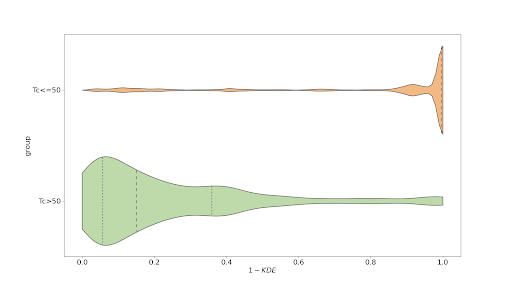
\includegraphics[width=0.95\textwidth]{figures/cond_high_chemical.png}
        \caption{Violin}
        \label{cond_high_chemical}
        \end{figure}

        \item From the domains assigned in our methods section, we acquire the PR curve shown in Figure~\ref{cond_high_chemical_pr}.

        \begin{figure}[H]
        \centering
        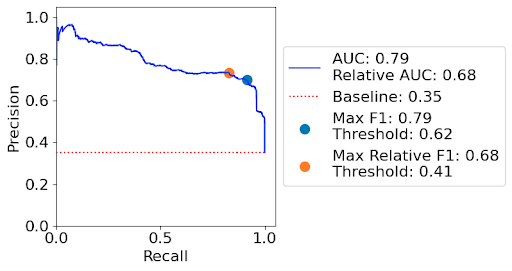
\includegraphics[width=0.95\textwidth]{figures/cond_high_chemical_pr.png}
        \caption{PR - Need to update this figure. Acts as placeholder.}
        \label{cond_high_chemical_pr}
        \end{figure}
        
        \item Figure~\ref{cond_low_chemical} has the violin plot for when we treat the majority of leave out data as $T_{high}$. Unfortunately, our $D$ measure does not show much difference in median values between $T_{low}$ and $T_{high}$. No ``good'' models can be constructed from these super conduction data. Hence, we believe our spatial measure will break down in this limit.

        \begin{figure}[H]
        \centering
        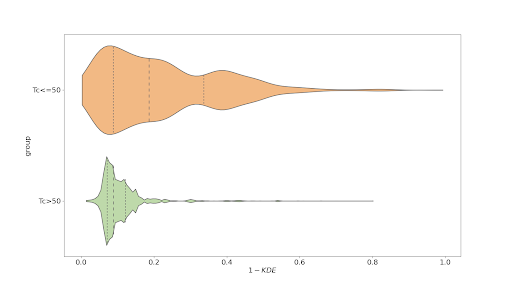
\includegraphics[width=0.95\textwidth]{figures/cond_low_chemical.png}
        \caption{Violin}
        \label{cond_low_chemical}
        \end{figure}

        \item From the domains assigned in our methods section, we acquire the PR curve shown in Figure~\ref{cond_low_chemical_pr}.

        \begin{figure}[H]
        \centering
        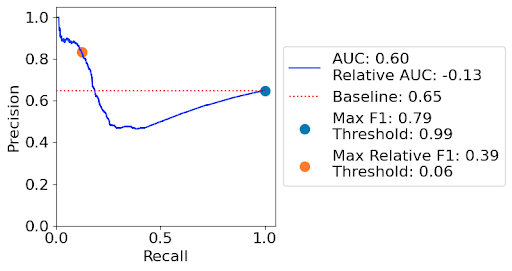
\includegraphics[width=0.95\textwidth]{figures/cond_low_chemical_pr.png}
        \caption{PR - Need to update this figure. Acts as placeholder.}
        \label{cond_low_chemical_pr}
        \end{figure}

    \end{enumerate}

    \item Numerical Single Assessment

    \begin{enumerate}

        \item Aggregated data from numerical tests are shown in Figure~\ref{cond_single}. Unusually, absolute residuals grow initially, but then decrease at $D$ is at its highest.

        \begin{figure}[H]
        \centering
        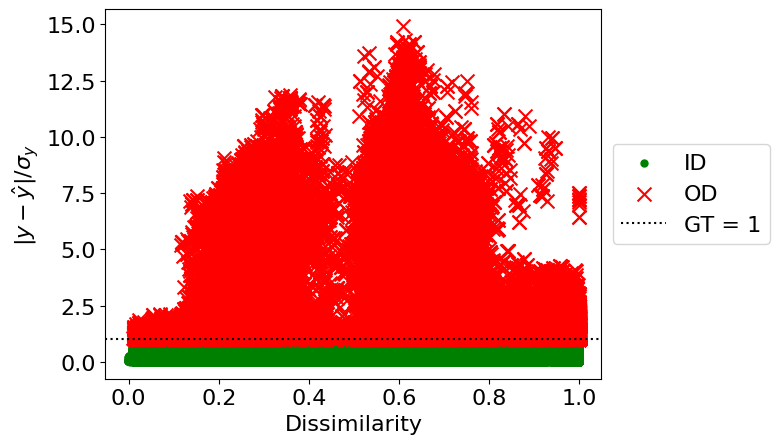
\includegraphics[width=0.95\textwidth]{figures/cond_single.png}
        \caption{Numerical}
        \label{cond_single}
        \end{figure}

        \item The associated precision recall curve is shown in Figure~\ref{cond_single_pr}.

        \begin{figure}[H]
        \centering
        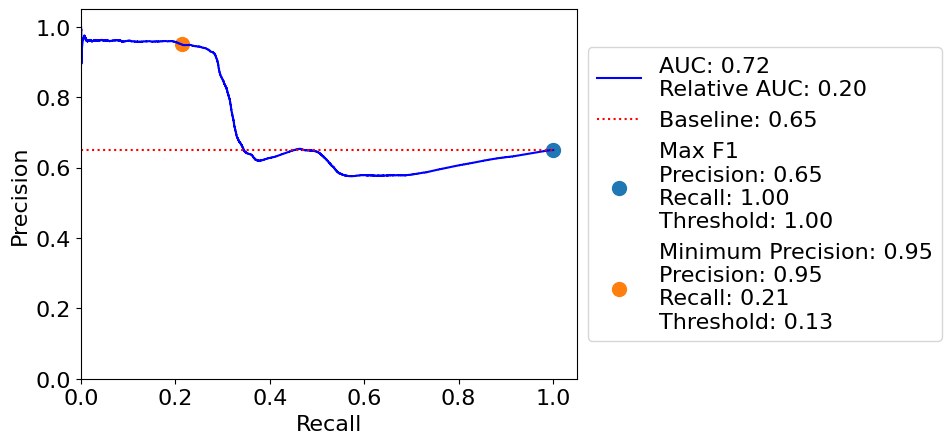
\includegraphics[width=0.95\textwidth]{figures/cond_single_pr.png}
        \caption{PR}
        \label{cond_single_pr}
        \end{figure}
    \end{enumerate}

    \item Numerical Statistical Assessment

    \begin{enumerate}
        \item We bin our data with respect to our $D$ score into 10 bins of with an equal number of points.

        \item We compare how z-score for each bin compare to a standard normal distribution (miscalibration area) and is sown in Figure~\ref{cond_stat}. Miscalibration area is greater to the right of around 0.2 compared to the left.

        \begin{figure}[H]
        \centering
        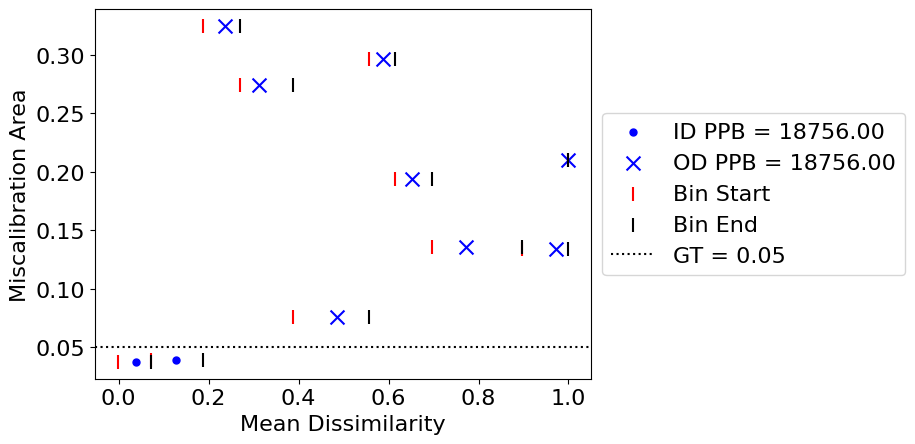
\includegraphics[width=0.95\textwidth]{figures/cond_stat.png}
        \caption{Numerical}
        \label{cond_stat}
        \end{figure}

        \item Our $D$ measure perfectly separates ID from OD data in this case in Figure~\ref{cond_stat_pr}.

        \begin{figure}[H]
        \centering
        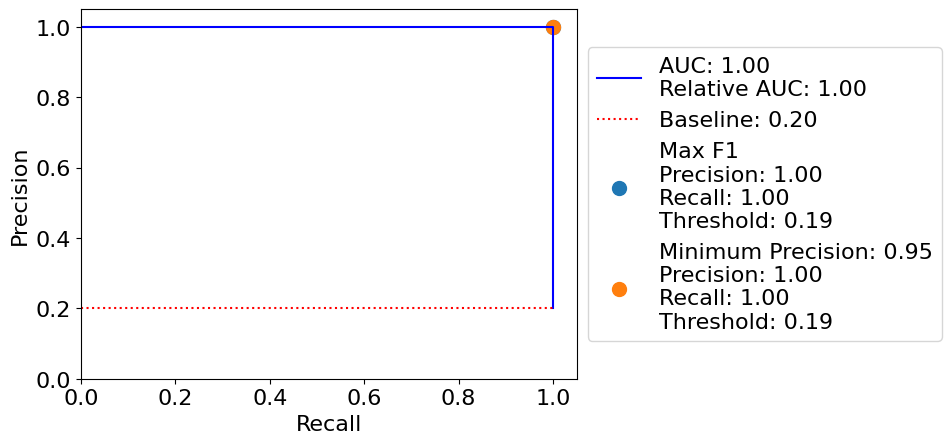
\includegraphics[width=0.95\textwidth]{figures/cond_stat_pr.png}
        \caption{PR}
        \label{cond_stat_pr}
        \end{figure}
        
    \end{enumerate}
    
\end{enumerate}

\subsection{Friedman}

\begin{enumerate}
    \item Numerical Single Assessment

    \begin{enumerate}

        \item Aggregated data from numerical tests are shown in Figure~\ref{friedman_single}.

        \begin{figure}[H]
        \centering
        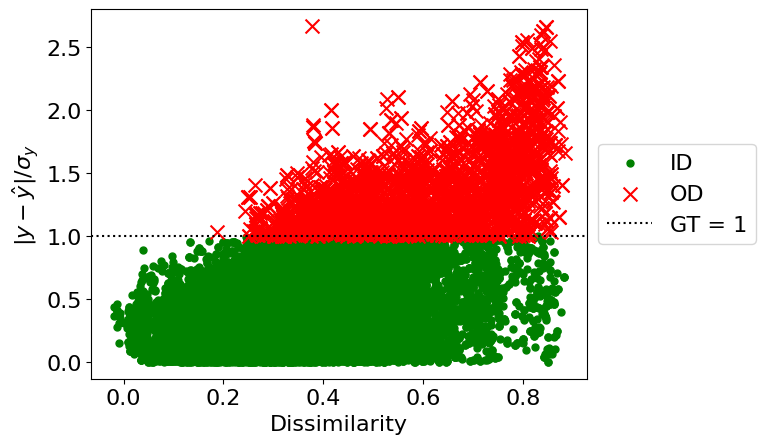
\includegraphics[width=0.95\textwidth]{figures/friedman_single.png}
        \caption{Numerical}
        \label{friedman_single}
        \end{figure}

        \item The associated precision recall curve is shown in Figure~\ref{friedman_single_pr}.

        \begin{figure}[H]
        \centering
        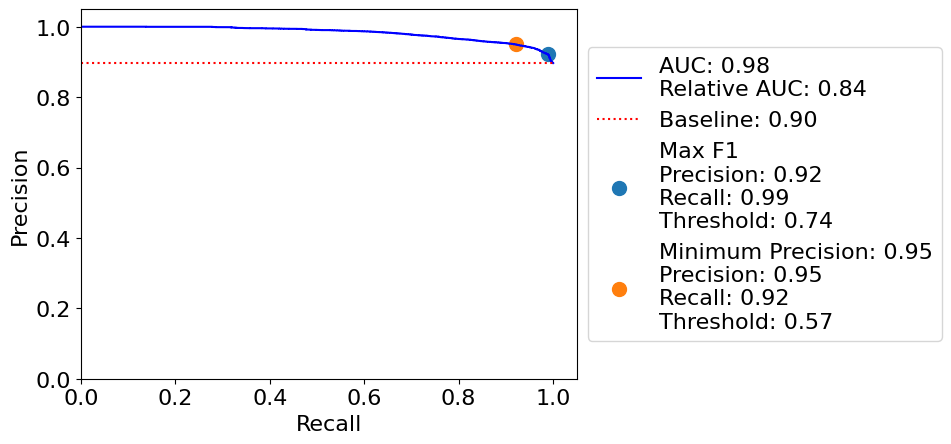
\includegraphics[width=0.95\textwidth]{figures/friedman_single_pr.png}
        \caption{PR}
        \label{friedman_single_pr}
        \end{figure}
    \end{enumerate}

    \item Numerical Statistical Assessment
    
    \begin{enumerate}
        \item We bin our data with respect to our $D$ score into 10 bins of with an equal number of points.

        \item We compare how z-score for each bin compare to a standard normal distribution (miscalibration area) and is sown in Figure~\ref{friedman_stat}. Miscalibration area First decreases until around 0.19 and then being to increase after around 0.29. 

        \begin{figure}[H]
        \centering
        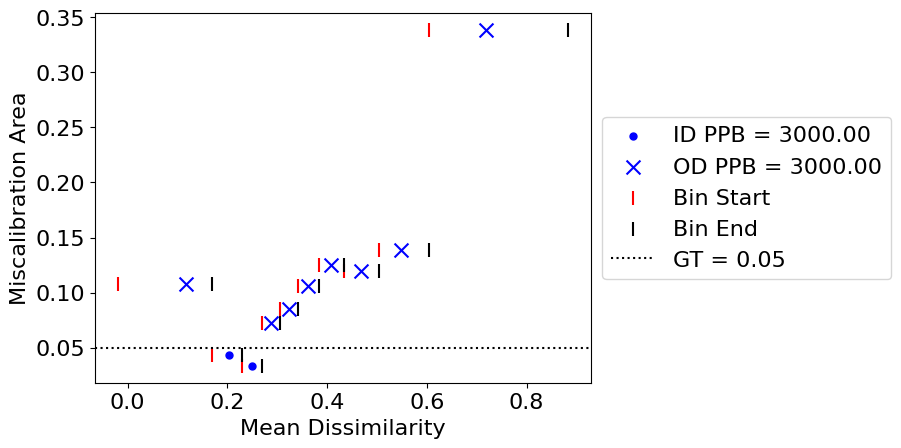
\includegraphics[width=0.95\textwidth]{figures/friedman_stat.png}
        \caption{Numerical}
        \label{friedman_stat}
        \end{figure}

        \item Unlike all of our previous tests, our $D$ measure does not perfectly separates ID from OD data Figure~\ref{friedman_stat_pr}. Unusually, our closest interval of points are miscalibrated.

        \begin{figure}[H]
        \centering
        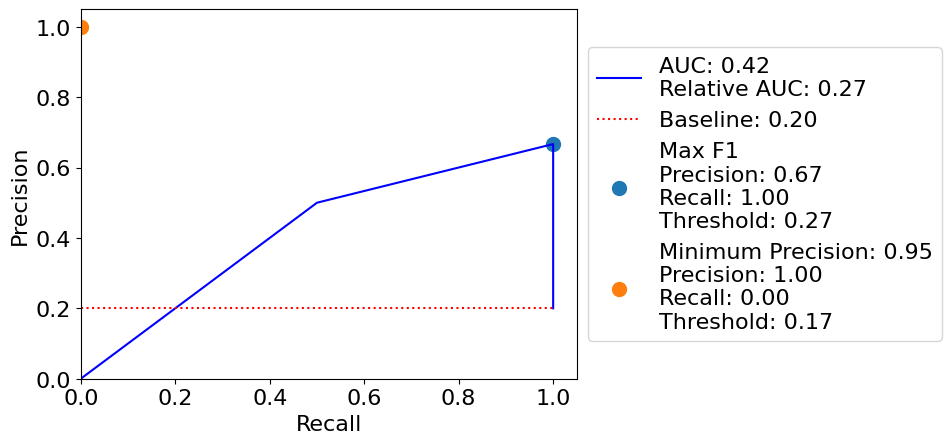
\includegraphics[width=0.95\textwidth]{figures/friedman_stat_pr.png}
        \caption{PR}
        \label{friedman_stat_pr}
        \end{figure}
        
    \end{enumerate}

\subsection{Aggregate Results}

\begin{enumerate}
    \item Include all major results in a table similar to that in Table~\ref{aggregate_results}.
    \item We note that for the vast majority of tests and data sets, our $D$ is a success.
\end{enumerate}

\begin{table}[H]
\begin{tabular}{|l|l|l|l|l|l|}
\hline
\textbf{Data} & \textbf{Domain}       & \textbf{Baseline} & \textbf{AUC} & \textbf{Relative AUC} & \textbf{Max F1} \\ \hline
diffusion     & chemical              &                   &              &                       &                 \\ \hline
diffusion     & single numerical      &                   &              &                       &                 \\ \hline
diffusion     & statistical numerical &                   &              &                       &                 \\ \hline
...           &                       &                   &              &                       &                 \\ \hline
\end{tabular}
\caption{All results}
\label{aggregate_results}
\end{table}

\end{enumerate}